\section{Technical implementation and details}

\subsection{FIDO2}

As already briefly introduced in \autoref{subsec:fido_alliance}, the \gls{fido}2 project is a joint efforts of the \gls{w3c} and the \gls{fido} alliance. It consists of the JavaScript standard, the \wa{}, and the \gls{ctap}. The \wa{} is standardized and managed by the \gls{w3c}, while the \gls{ctap} is authored by the \gls{fido} alliance. However, the \gls{fido} alliance also initially developed the \wa{} under the name \gls{fido} 2.0 before officially handing it over to the \gls{w3c}.

\begin{figure}[hbt]
	\centering
	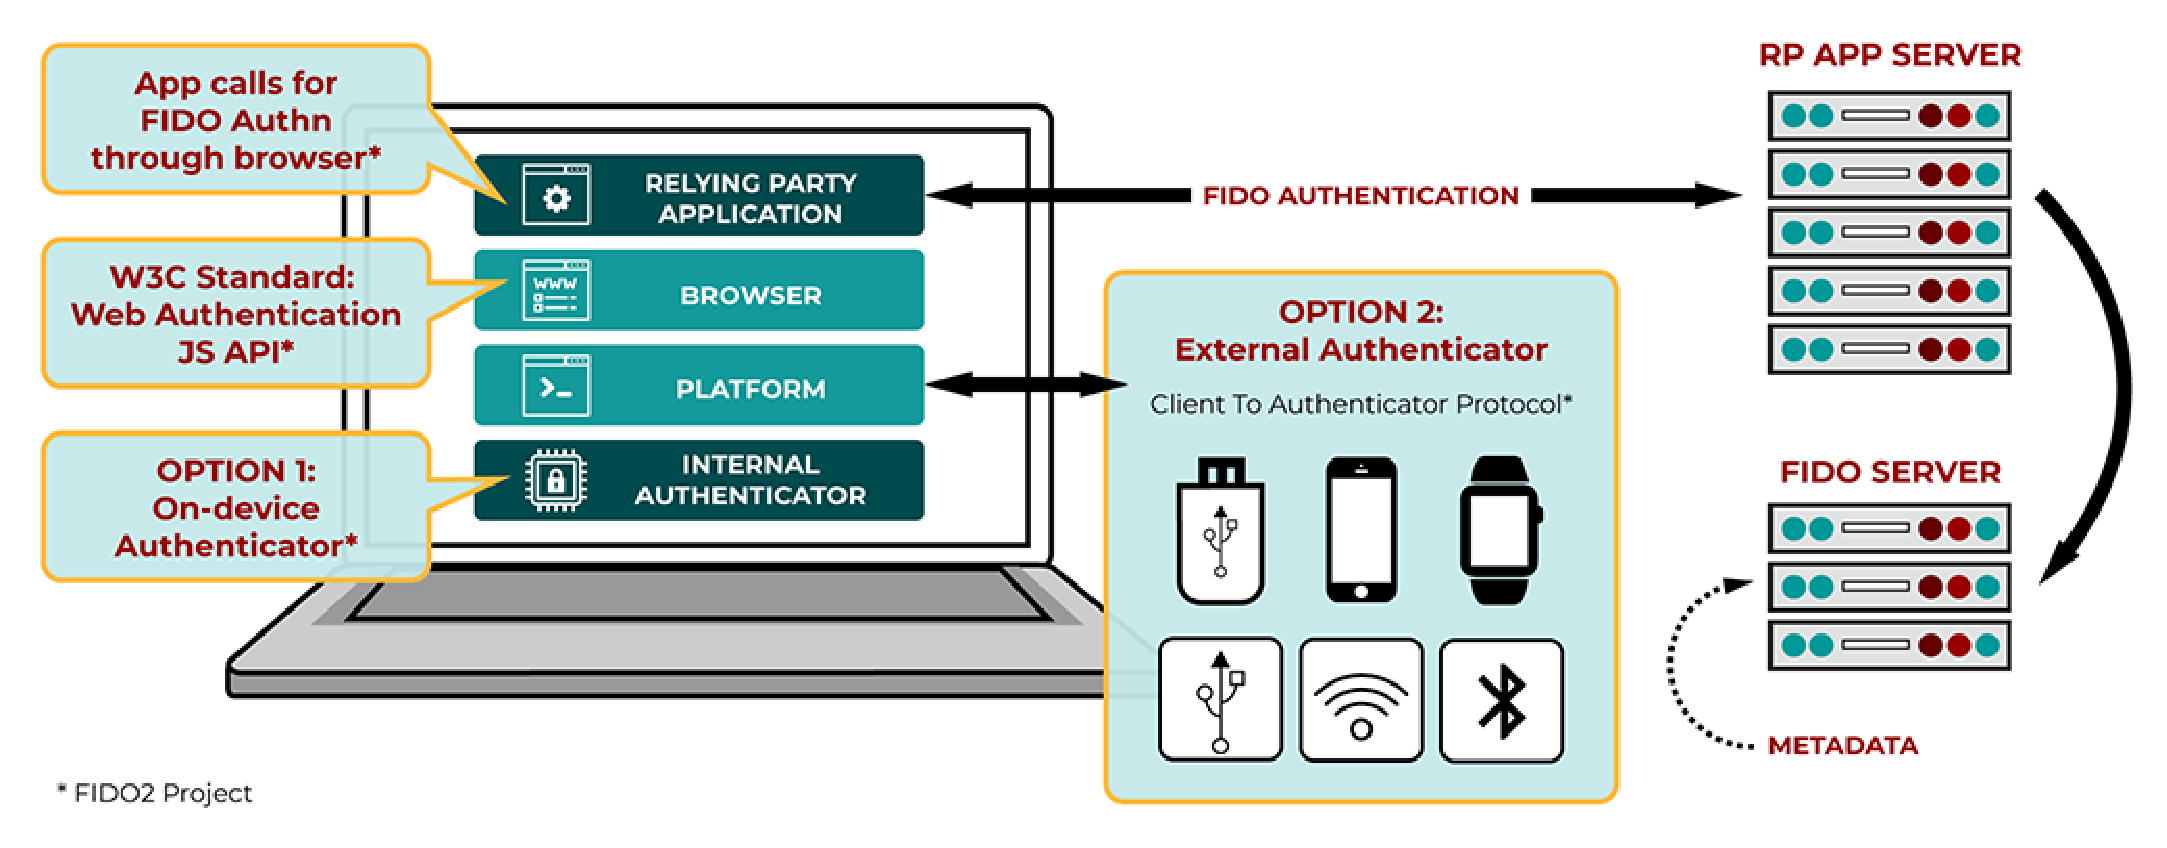
\includegraphics[width=\textwidth]{pics/FIDO2-Graphic-v2}
	\caption[\gls{fido}2 architecture overview]{\gls{fido}2 architecture overview\footnotemark}
	\label{fig:fido2_architecture}
\end{figure}
\footcitetext[Source: https://fidoalliance.org/specifications/][4]{uaf-overview}

\autoref{fig:fido2_architecture} shows the overview of the \gls{fido}2 project. A noteworthy change is the possibility to use either a \textit{roaming}, i.e., external authenticator or an authenticator that is built into the device.

\subsection{Client to Authenticator Protocol 2}

The \glsfirst{ctap} 2 is based on the \gls{u2f} protocol version 1.2 and defines three parts:

\begin{enumerate}
	\item the authenticator \gls{api}
	\item message encoding
	\item transport-specifc binding
\end{enumerate}

The key methods of the authenticator \gls{api} are explained in more detail below. Message encoding describes the process of encoding the corresponding message in a binary encoding called \gls{cbor} that is suitable for, e.g., the transport over \gls{ble}, because plain text string and \gls{json} objects might be too big. The transport-specific bindings define the required transformation and bindings in order to comply with the transport protocol specifications.

\subsubsection{Registration}



\subsubsection{Authentication}

\subsubsection{Factory reset}

Like the \gls{uaf} protocol, but in contrast to the \gls{u2f} specification, \gls{ctap} does again define a method to completely factory reset the authenticator in order to de-register every user account on it. To avoid accidental deletion, the protocol specifies that the authenticator may ask for user confirmation. 

\subsection{Web Authentication API}

The \wa{} is backwards compatible to the \gls{u2f} compatible, thus making every security token that is usable for \gls{u2f} compatible with the \wa, too.